\section{\textsc{Spaghetti spinach carbonara with poached egg}}

\subsection*{Ingredients for 2 portions:}

\begin{tabular}{p{7.5cm} p{7.5cm}}
	& \\
	200g spaghetti & 2 handfull fresh spinach \\
	\sfrac{1}{2} diced onion & \sfrac{1}{2} garlic clove \\
  40g bacon & 3 eggs \\
  100ml page & dash of vinegar \\
  salt, pepper & 1tbsp sunflower oil
\end{tabular}

\subsection*{Serving suggestion:}

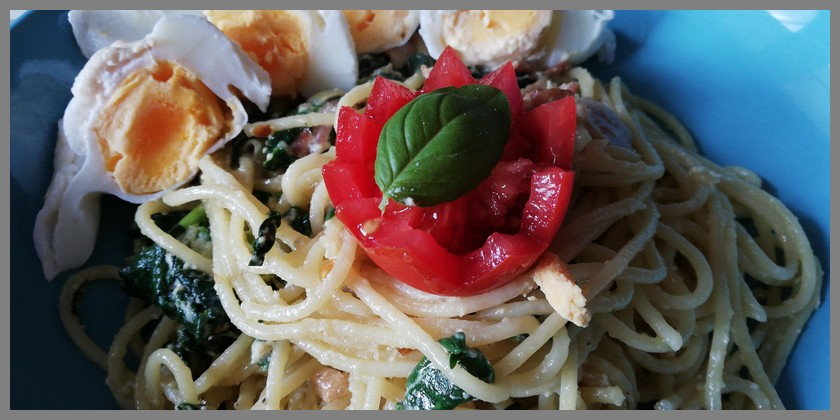
\includegraphics[width=\textwidth]{img/spaghetti_ei.jpeg} \cite{eicorbonara}

\subsection*{How it's done:}

\begin{tabular}{p{15cm}}
	\\
  First cook the spaghetti according to the package instructions al denkte.\\
  Then cut the bacon into 4cm long strips.\\
  Put the oil in a hot pan and fry the onions and bacon until crispy.\\
  After about 5 minutes, add the spinach and fry until it collapses. Season with salt and pepper.\\
  Now add the spaghetti to a larger pan (or roaster).\\
  Pour the cream into a measuring cup and add an egg. Beat both.\\
  Pour over the spinach mix and reduce everything.\\
  In another top bring about 1,5l water to the boil.\\
  Turn down the heat so that the water only boils slightly. Add the vinegar.\\
  Whip an egg in a flat cup. Make sure that the egg yolk remains undamaged.\\
  From the cup, let the egg slide slowly into the hot water. Poach for 6-7 minutes.\\
  Repeat with another egg.
\end{tabular}
